\subsection{Setup}\label{sec:setup}
The tests are, as mentioned in Section \ref{sec:groupgeneration}, going to be performed on groups with member sizes of 4, 8, 12, 16, 20, and 40, and there are going to be 1000 random generated groups of each size. Throughout these tests we have decided to assign $k$ the size 10. In Figure \ref{fig:setup}, we see the how lists of individual recommendations for a group of size $u$ will be put through an aggregation method before outputting a list of k ranked items.
\begin{figure}[h]
\centering
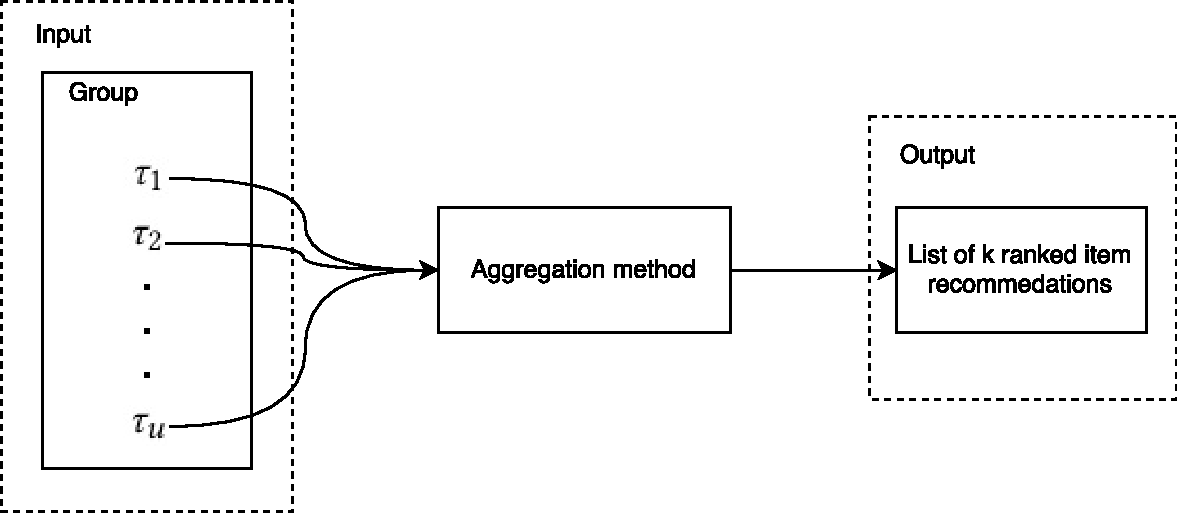
\includegraphics[scale=.4]{graphics/setup}
\caption{Concept of the test setup. Aggregation methods take in multiple lists and returns a list of recommendations to be evaluated.}\label{fig:composition}
\label{fig:setup}
\end{figure}
\subsubsection{T-test}
We made paired t-tests for all methods. Each method is compared with each of the other methods for all measures. The t-test outputs a p-value, which is the probability that the difference between two sets of results is coincidental. At $0.05$ or lower, it is considered that there is statistically significant difference in the means of the two sets.\note{Citation}
\subsubsection{Ranking Measures}
To measure our rankings, we use nDCG, Rating nDCG, KTD and SFD, each covered in Section \ref{sec:ranking}\note{missing label}. The way we are going to present the results of these tests are by finding the average score across the 1000 groups across a group size for each method and measure. What this means is the we first find an average score for a group. Then we find the average for all the groups, and that is the returned value for the measure.